% Options for packages loaded elsewhere
% Options for packages loaded elsewhere
\PassOptionsToPackage{unicode}{hyperref}
\PassOptionsToPackage{hyphens}{url}
\PassOptionsToPackage{dvipsnames,svgnames,x11names}{xcolor}
%
\documentclass[
  letterpaper,
  DIV=11,
  numbers=noendperiod]{scrartcl}
\usepackage{xcolor}
\usepackage{amsmath,amssymb}
\setcounter{secnumdepth}{-\maxdimen} % remove section numbering
\usepackage{iftex}
\ifPDFTeX
  \usepackage[T1]{fontenc}
  \usepackage[utf8]{inputenc}
  \usepackage{textcomp} % provide euro and other symbols
\else % if luatex or xetex
  \usepackage{unicode-math} % this also loads fontspec
  \defaultfontfeatures{Scale=MatchLowercase}
  \defaultfontfeatures[\rmfamily]{Ligatures=TeX,Scale=1}
\fi
\usepackage{lmodern}
\ifPDFTeX\else
  % xetex/luatex font selection
\fi
% Use upquote if available, for straight quotes in verbatim environments
\IfFileExists{upquote.sty}{\usepackage{upquote}}{}
\IfFileExists{microtype.sty}{% use microtype if available
  \usepackage[]{microtype}
  \UseMicrotypeSet[protrusion]{basicmath} % disable protrusion for tt fonts
}{}
\makeatletter
\@ifundefined{KOMAClassName}{% if non-KOMA class
  \IfFileExists{parskip.sty}{%
    \usepackage{parskip}
  }{% else
    \setlength{\parindent}{0pt}
    \setlength{\parskip}{6pt plus 2pt minus 1pt}}
}{% if KOMA class
  \KOMAoptions{parskip=half}}
\makeatother
% Make \paragraph and \subparagraph free-standing
\makeatletter
\ifx\paragraph\undefined\else
  \let\oldparagraph\paragraph
  \renewcommand{\paragraph}{
    \@ifstar
      \xxxParagraphStar
      \xxxParagraphNoStar
  }
  \newcommand{\xxxParagraphStar}[1]{\oldparagraph*{#1}\mbox{}}
  \newcommand{\xxxParagraphNoStar}[1]{\oldparagraph{#1}\mbox{}}
\fi
\ifx\subparagraph\undefined\else
  \let\oldsubparagraph\subparagraph
  \renewcommand{\subparagraph}{
    \@ifstar
      \xxxSubParagraphStar
      \xxxSubParagraphNoStar
  }
  \newcommand{\xxxSubParagraphStar}[1]{\oldsubparagraph*{#1}\mbox{}}
  \newcommand{\xxxSubParagraphNoStar}[1]{\oldsubparagraph{#1}\mbox{}}
\fi
\makeatother

\usepackage{color}
\usepackage{fancyvrb}
\newcommand{\VerbBar}{|}
\newcommand{\VERB}{\Verb[commandchars=\\\{\}]}
\DefineVerbatimEnvironment{Highlighting}{Verbatim}{commandchars=\\\{\}}
% Add ',fontsize=\small' for more characters per line
\usepackage{framed}
\definecolor{shadecolor}{RGB}{241,243,245}
\newenvironment{Shaded}{\begin{snugshade}}{\end{snugshade}}
\newcommand{\AlertTok}[1]{\textcolor[rgb]{0.68,0.00,0.00}{#1}}
\newcommand{\AnnotationTok}[1]{\textcolor[rgb]{0.37,0.37,0.37}{#1}}
\newcommand{\AttributeTok}[1]{\textcolor[rgb]{0.40,0.45,0.13}{#1}}
\newcommand{\BaseNTok}[1]{\textcolor[rgb]{0.68,0.00,0.00}{#1}}
\newcommand{\BuiltInTok}[1]{\textcolor[rgb]{0.00,0.23,0.31}{#1}}
\newcommand{\CharTok}[1]{\textcolor[rgb]{0.13,0.47,0.30}{#1}}
\newcommand{\CommentTok}[1]{\textcolor[rgb]{0.37,0.37,0.37}{#1}}
\newcommand{\CommentVarTok}[1]{\textcolor[rgb]{0.37,0.37,0.37}{\textit{#1}}}
\newcommand{\ConstantTok}[1]{\textcolor[rgb]{0.56,0.35,0.01}{#1}}
\newcommand{\ControlFlowTok}[1]{\textcolor[rgb]{0.00,0.23,0.31}{\textbf{#1}}}
\newcommand{\DataTypeTok}[1]{\textcolor[rgb]{0.68,0.00,0.00}{#1}}
\newcommand{\DecValTok}[1]{\textcolor[rgb]{0.68,0.00,0.00}{#1}}
\newcommand{\DocumentationTok}[1]{\textcolor[rgb]{0.37,0.37,0.37}{\textit{#1}}}
\newcommand{\ErrorTok}[1]{\textcolor[rgb]{0.68,0.00,0.00}{#1}}
\newcommand{\ExtensionTok}[1]{\textcolor[rgb]{0.00,0.23,0.31}{#1}}
\newcommand{\FloatTok}[1]{\textcolor[rgb]{0.68,0.00,0.00}{#1}}
\newcommand{\FunctionTok}[1]{\textcolor[rgb]{0.28,0.35,0.67}{#1}}
\newcommand{\ImportTok}[1]{\textcolor[rgb]{0.00,0.46,0.62}{#1}}
\newcommand{\InformationTok}[1]{\textcolor[rgb]{0.37,0.37,0.37}{#1}}
\newcommand{\KeywordTok}[1]{\textcolor[rgb]{0.00,0.23,0.31}{\textbf{#1}}}
\newcommand{\NormalTok}[1]{\textcolor[rgb]{0.00,0.23,0.31}{#1}}
\newcommand{\OperatorTok}[1]{\textcolor[rgb]{0.37,0.37,0.37}{#1}}
\newcommand{\OtherTok}[1]{\textcolor[rgb]{0.00,0.23,0.31}{#1}}
\newcommand{\PreprocessorTok}[1]{\textcolor[rgb]{0.68,0.00,0.00}{#1}}
\newcommand{\RegionMarkerTok}[1]{\textcolor[rgb]{0.00,0.23,0.31}{#1}}
\newcommand{\SpecialCharTok}[1]{\textcolor[rgb]{0.37,0.37,0.37}{#1}}
\newcommand{\SpecialStringTok}[1]{\textcolor[rgb]{0.13,0.47,0.30}{#1}}
\newcommand{\StringTok}[1]{\textcolor[rgb]{0.13,0.47,0.30}{#1}}
\newcommand{\VariableTok}[1]{\textcolor[rgb]{0.07,0.07,0.07}{#1}}
\newcommand{\VerbatimStringTok}[1]{\textcolor[rgb]{0.13,0.47,0.30}{#1}}
\newcommand{\WarningTok}[1]{\textcolor[rgb]{0.37,0.37,0.37}{\textit{#1}}}

\usepackage{longtable,booktabs,array}
\usepackage{calc} % for calculating minipage widths
% Correct order of tables after \paragraph or \subparagraph
\usepackage{etoolbox}
\makeatletter
\patchcmd\longtable{\par}{\if@noskipsec\mbox{}\fi\par}{}{}
\makeatother
% Allow footnotes in longtable head/foot
\IfFileExists{footnotehyper.sty}{\usepackage{footnotehyper}}{\usepackage{footnote}}
\makesavenoteenv{longtable}
\usepackage{graphicx}
\makeatletter
\newsavebox\pandoc@box
\newcommand*\pandocbounded[1]{% scales image to fit in text height/width
  \sbox\pandoc@box{#1}%
  \Gscale@div\@tempa{\textheight}{\dimexpr\ht\pandoc@box+\dp\pandoc@box\relax}%
  \Gscale@div\@tempb{\linewidth}{\wd\pandoc@box}%
  \ifdim\@tempb\p@<\@tempa\p@\let\@tempa\@tempb\fi% select the smaller of both
  \ifdim\@tempa\p@<\p@\scalebox{\@tempa}{\usebox\pandoc@box}%
  \else\usebox{\pandoc@box}%
  \fi%
}
% Set default figure placement to htbp
\def\fps@figure{htbp}
\makeatother





\setlength{\emergencystretch}{3em} % prevent overfull lines

\providecommand{\tightlist}{%
  \setlength{\itemsep}{0pt}\setlength{\parskip}{0pt}}



 


\KOMAoption{captions}{tableheading}
\makeatletter
\@ifpackageloaded{tcolorbox}{}{\usepackage[skins,breakable]{tcolorbox}}
\@ifpackageloaded{fontawesome5}{}{\usepackage{fontawesome5}}
\definecolor{quarto-callout-color}{HTML}{909090}
\definecolor{quarto-callout-note-color}{HTML}{0758E5}
\definecolor{quarto-callout-important-color}{HTML}{CC1914}
\definecolor{quarto-callout-warning-color}{HTML}{EB9113}
\definecolor{quarto-callout-tip-color}{HTML}{00A047}
\definecolor{quarto-callout-caution-color}{HTML}{FC5300}
\definecolor{quarto-callout-color-frame}{HTML}{acacac}
\definecolor{quarto-callout-note-color-frame}{HTML}{4582ec}
\definecolor{quarto-callout-important-color-frame}{HTML}{d9534f}
\definecolor{quarto-callout-warning-color-frame}{HTML}{f0ad4e}
\definecolor{quarto-callout-tip-color-frame}{HTML}{02b875}
\definecolor{quarto-callout-caution-color-frame}{HTML}{fd7e14}
\makeatother
\makeatletter
\@ifpackageloaded{caption}{}{\usepackage{caption}}
\AtBeginDocument{%
\ifdefined\contentsname
  \renewcommand*\contentsname{Table of contents}
\else
  \newcommand\contentsname{Table of contents}
\fi
\ifdefined\listfigurename
  \renewcommand*\listfigurename{List of Figures}
\else
  \newcommand\listfigurename{List of Figures}
\fi
\ifdefined\listtablename
  \renewcommand*\listtablename{List of Tables}
\else
  \newcommand\listtablename{List of Tables}
\fi
\ifdefined\figurename
  \renewcommand*\figurename{Figure}
\else
  \newcommand\figurename{Figure}
\fi
\ifdefined\tablename
  \renewcommand*\tablename{Table}
\else
  \newcommand\tablename{Table}
\fi
}
\@ifpackageloaded{float}{}{\usepackage{float}}
\floatstyle{ruled}
\@ifundefined{c@chapter}{\newfloat{codelisting}{h}{lop}}{\newfloat{codelisting}{h}{lop}[chapter]}
\floatname{codelisting}{Listing}
\newcommand*\listoflistings{\listof{codelisting}{List of Listings}}
\makeatother
\makeatletter
\makeatother
\makeatletter
\@ifpackageloaded{caption}{}{\usepackage{caption}}
\@ifpackageloaded{subcaption}{}{\usepackage{subcaption}}
\makeatother
\usepackage{bookmark}
\IfFileExists{xurl.sty}{\usepackage{xurl}}{} % add URL line breaks if available
\urlstyle{same}
\hypersetup{
  pdftitle={Object-Oriented Matplotlib Challenge},
  colorlinks=true,
  linkcolor={blue},
  filecolor={Maroon},
  citecolor={Blue},
  urlcolor={Blue},
  pdfcreator={LaTeX via pandoc}}


\title{Object-Oriented Matplotlib Challenge}
\usepackage{etoolbox}
\makeatletter
\providecommand{\subtitle}[1]{% add subtitle to \maketitle
  \apptocmd{\@title}{\par {\large #1 \par}}{}{}
}
\makeatother
\subtitle{Mastering the Four Stages of Data Visualization}
\author{}
\date{}
\begin{document}
\maketitle


\section{🎯 Object-Oriented Matplotlib Challenge - The Four Stages of
Data
Visualization}\label{object-oriented-matplotlib-challenge---the-four-stages-of-data-visualization}

\begin{tcolorbox}[enhanced jigsaw, rightrule=.15mm, coltitle=black, colbacktitle=quarto-callout-important-color!10!white, opacitybacktitle=0.6, arc=.35mm, leftrule=.75mm, colback=white, title=\textcolor{quarto-callout-important-color}{\faExclamation}\hspace{0.5em}{📊 Challenge Requirements}, colframe=quarto-callout-important-color-frame, bottomrule=.15mm, left=2mm, opacityback=0, toptitle=1mm, titlerule=0mm, toprule=.15mm, bottomtitle=1mm, breakable]

\begin{itemize}
\tightlist
\item
  Complete all discussion questions for the four stages of visualization
\item
  Create professional visualizations using object-oriented matplotlib
\item
  Demonstrate mastery of the Grammar of Graphics
\item
  See \hyperref[student-analysis-section]{Student Analysis Section} for
  detailed requirements
\end{itemize}

\end{tcolorbox}

\subsection{The Problem: Mastering Object-Oriented Matplotlib Through
the Four
Stages}\label{the-problem-mastering-object-oriented-matplotlib-through-the-four-stages}

\textbf{Core Question:} How can we create compelling, professional data
visualizations using object-oriented matplotlib and the four stages of
visualization?

\textbf{The Challenge:} Real-world data visualization requires more than
just plotting data - it requires a systematic approach that transforms
raw data into compelling stories. The four stages framework provides a
proven methodology for creating visualizations that inform, persuade,
and inspire action.

\textbf{Our Approach:} We'll work with baseball stadium data to
investigate whether Coors Field in Denver, Colorado is truly the most
run-friendly ballpark in Major League Baseball. This investigation will
take us through all four stages of visualization, demonstrating
object-oriented matplotlib techniques along the way.

\begin{tcolorbox}[enhanced jigsaw, rightrule=.15mm, coltitle=black, colbacktitle=quarto-callout-warning-color!10!white, opacitybacktitle=0.6, arc=.35mm, leftrule=.75mm, colback=white, title=\textcolor{quarto-callout-warning-color}{\faExclamationTriangle}\hspace{0.5em}{⚠️ AI Partnership Required}, colframe=quarto-callout-warning-color-frame, bottomrule=.15mm, left=2mm, opacityback=0, toptitle=1mm, titlerule=0mm, toprule=.15mm, bottomtitle=1mm, breakable]

This challenge pushes boundaries intentionally. You'll tackle problems
that normally require weeks of study, but with Cursor AI as your partner
(and your brain keeping it honest), you can accomplish more than you
thought possible.

\textbf{The new reality:} The four stages of competence are Ignorance →
Awareness → Learning → Mastery. AI lets us produce Mastery-level work
while operating primarily in the Awareness stage. I focus on awareness
training, you leverage AI for execution, and together we create outputs
that used to require years of dedicated study.

\end{tcolorbox}

\subsection{The Four Stages of Data
Visualization}\label{the-four-stages-of-data-visualization}

The four essential stages for creating effective visualizations are:

\begin{enumerate}
\def\labelenumi{\arabic{enumi}.}
\tightlist
\item
  \textbf{Stage 1: Declaration of Purpose} - Define your message and
  audience
\item
  \textbf{Stage 2: Curation of Content} - Gather and create all
  necessary data
\item
  \textbf{Stage 3: Structuring of Visual Mappings} - Choose geometry and
  aesthetics
\item
  \textbf{Stage 4: Formatting for Your Audience} - Polish for
  professional presentation
\end{enumerate}

\subsection{Data and Business Context}\label{data-and-business-context}

We analyze Major League Baseball stadium data to investigate whether
Coors Field in Denver, Colorado is truly the most run-friendly ballpark.
This dataset is ideal for our analysis because:

\begin{itemize}
\tightlist
\item
  \textbf{Real Business Question:} Sports analysts and fans want to
  understand stadium effects on scoring
\item
  \textbf{Clear Hypothesis:} High altitude should make Coors Field more
  run-friendly
\item
  \textbf{Multiple Metrics:} We can analyze both total runs and home
  runs
\item
  \textbf{Visualization Practice:} Perfect for demonstrating all four
  stages of visualization
\end{itemize}

\subsection{Data Loading and Initial
Exploration}\label{data-loading-and-initial-exploration}

Let's start by loading the baseball data and understanding what we're
working with.

\phantomsection\label{load-data}
\begin{Shaded}
\begin{Highlighting}[]
\ImportTok{import}\NormalTok{ matplotlib.pyplot }\ImportTok{as}\NormalTok{ plt}
\ImportTok{import}\NormalTok{ pandas }\ImportTok{as}\NormalTok{ pd}
\ImportTok{import}\NormalTok{ numpy }\ImportTok{as}\NormalTok{ np}
\ImportTok{import}\NormalTok{ seaborn }\ImportTok{as}\NormalTok{ sns}

\CommentTok{\# Load 2010 baseball season data}
\NormalTok{df2010 }\OperatorTok{=}\NormalTok{ pd.read\_csv(}\StringTok{"baseball10.csv"}\NormalTok{)}

\CommentTok{\# Load 2021 baseball season data for comparison}
\NormalTok{df2021 }\OperatorTok{=}\NormalTok{ pd.read\_csv(}\StringTok{"baseball21.csv"}\NormalTok{)}

\BuiltInTok{print}\NormalTok{(}\StringTok{"2010 data shape:"}\NormalTok{, df2010.shape)}
\BuiltInTok{print}\NormalTok{(}\StringTok{"2021 data shape:"}\NormalTok{, df2021.shape)}
\BuiltInTok{print}\NormalTok{(}\StringTok{"}\CharTok{\textbackslash{}n}\StringTok{2010 data columns:"}\NormalTok{, df2010.columns.tolist())}
\BuiltInTok{print}\NormalTok{(}\StringTok{"}\CharTok{\textbackslash{}n}\StringTok{First few rows of 2010 data:"}\NormalTok{)}
\BuiltInTok{print}\NormalTok{(df2010.head())}
\end{Highlighting}
\end{Shaded}

\begin{verbatim}
2010 data shape: (2430, 7)
2021 data shape: (2429, 7)

2010 data columns: ['date', 'visiting', 'home', 'visScore', 'homeScore', 'visHR', 'homeHR']

First few rows of 2010 data:
       date visiting home  visScore  homeScore  visHR  homeHR
0  20100404      NYA  BOS         7          9      2       1
1  20100405      MIN  ANA         3          6      1       3
2  20100405      CLE  CHA         0          6      0       2
3  20100405      DET  KCA         8          4      0       1
4  20100405      SEA  OAK         5          3      1       0
\end{verbatim}

\begin{tcolorbox}[enhanced jigsaw, rightrule=.15mm, coltitle=black, colbacktitle=quarto-callout-note-color!10!white, opacitybacktitle=0.6, arc=.35mm, leftrule=.75mm, colback=white, title=\textcolor{quarto-callout-note-color}{\faInfo}\hspace{0.5em}{💡 Understanding the Data}, colframe=quarto-callout-note-color-frame, bottomrule=.15mm, left=2mm, opacityback=0, toptitle=1mm, titlerule=0mm, toprule=.15mm, bottomtitle=1mm, breakable]

\textbf{Baseball Game Data:} Contains information about each game,
including: - \texttt{home}: Home team (3-letter code) -
\texttt{visiting}: Visiting team (3-letter code) - \texttt{homeScore}:
Runs scored by home team - \texttt{visScore}: Runs scored by visiting
team - \texttt{homeHR}: Home runs by home team - \texttt{visHR}: Home
runs by visiting team - \texttt{date}: Game date

\textbf{Business Questions We'll Answer:} 1. Is Coors Field (COL) the
most run-friendly ballpark in 2010? 2. How does this change in 2021? 3.
What's the difference between total runs and home runs by stadium?

\end{tcolorbox}

\subsection{Stage 1: Declaration of
Purpose}\label{stage-1-declaration-of-purpose}

\textbf{Mental Model:} Start with a clear message and bold title that
states your recommendation.

Our purpose is to investigate whether Coors Field in Denver, Colorado is
truly the most run-friendly baseball stadium in Major League Baseball.

\begin{tcolorbox}[enhanced jigsaw, rightrule=.15mm, coltitle=black, colbacktitle=quarto-callout-important-color!10!white, opacitybacktitle=0.6, arc=.35mm, leftrule=.75mm, colback=white, title=\textcolor{quarto-callout-important-color}{\faExclamation}\hspace{0.5em}{🤔 Discussion Questions: Stage 1 - Declaration of Purpose}, colframe=quarto-callout-important-color-frame, bottomrule=.15mm, left=2mm, opacityback=0, toptitle=1mm, titlerule=0mm, toprule=.15mm, bottomtitle=1mm, breakable]

\textbf{Question 1: Hypothesis Formation} - Why might high altitude
affect baseball performance? Is Coors Field affected by high altitude?

\end{tcolorbox}

\textbf{ANSWER:} At high altitude, the air is thinner, which means that
the ball travels farther. This is why Coors Field is known for being a
home run hitter's park.

\subsection{Stage 2: Curation of
Content}\label{stage-2-curation-of-content}

\textbf{Mental Model:} Gather and create all the data you need to
support your message.

Let's aggregate the data to get average runs per stadium:

\phantomsection\label{stage-2-content}
\begin{Shaded}
\begin{Highlighting}[]
\CommentTok{\# Stage 2: Curation of Content}
\CommentTok{\# Aggregate data to get average runs per stadium}

\CommentTok{\# Process 2010 data}
\NormalTok{avgDF\_2010 }\OperatorTok{=}\NormalTok{ (df2010}
\NormalTok{    .assign(totalRuns }\OperatorTok{=} \KeywordTok{lambda}\NormalTok{ df: df.homeScore }\OperatorTok{+}\NormalTok{ df.visScore)}
\NormalTok{    .assign(totalHR }\OperatorTok{=} \KeywordTok{lambda}\NormalTok{ df: df.homeHR }\OperatorTok{+}\NormalTok{ df.visHR)}
\NormalTok{    .drop(columns }\OperatorTok{=}\NormalTok{ [}\StringTok{\textquotesingle{}date\textquotesingle{}}\NormalTok{, }\StringTok{\textquotesingle{}visiting\textquotesingle{}}\NormalTok{])}
\NormalTok{    .groupby([}\StringTok{\textquotesingle{}home\textquotesingle{}}\NormalTok{], as\_index}\OperatorTok{=}\VariableTok{False}\NormalTok{)}
\NormalTok{    .mean()}
\NormalTok{)}

\CommentTok{\# Process 2021 data}
\NormalTok{avgDF\_2021 }\OperatorTok{=}\NormalTok{ (df2021}
\NormalTok{    .assign(totalRuns }\OperatorTok{=} \KeywordTok{lambda}\NormalTok{ df: df.homeScore }\OperatorTok{+}\NormalTok{ df.visScore)}
\NormalTok{    .assign(totalHR }\OperatorTok{=} \KeywordTok{lambda}\NormalTok{ df: df.homeHR }\OperatorTok{+}\NormalTok{ df.visHR)}
\NormalTok{    .drop(columns }\OperatorTok{=}\NormalTok{ [}\StringTok{\textquotesingle{}date\textquotesingle{}}\NormalTok{, }\StringTok{\textquotesingle{}visiting\textquotesingle{}}\NormalTok{])}
\NormalTok{    .groupby([}\StringTok{\textquotesingle{}home\textquotesingle{}}\NormalTok{], as\_index}\OperatorTok{=}\VariableTok{False}\NormalTok{)}
\NormalTok{    .mean()}
\NormalTok{)}

\BuiltInTok{print}\NormalTok{(}\StringTok{"2010 Stadium Averages (Top 5):"}\NormalTok{)}
\BuiltInTok{print}\NormalTok{(avgDF\_2010.head())}
\BuiltInTok{print}\NormalTok{(}\StringTok{"}\CharTok{\textbackslash{}n}\StringTok{2021 Stadium Averages (Top 5):"}\NormalTok{)}
\BuiltInTok{print}\NormalTok{(avgDF\_2021.head())}
\end{Highlighting}
\end{Shaded}

\begin{verbatim}
2010 Stadium Averages (Top 5):
  home  visScore  homeScore     visHR    homeHR  totalRuns   totalHR
0  ANA  3.975309   3.938272  0.839506  0.851852   7.913580  1.691358
1  ARI  5.049383   4.740741  1.271605  1.209877   9.790123  2.481481
2  ATL  3.641975   4.827160  0.740741  0.913580   8.469136  1.654321
3  BAL  5.111111   3.975309  1.308642  0.888889   9.086420  2.197531
4  BOS  4.851852   5.172840  0.876543  1.209877  10.024691  2.086420

2021 Stadium Averages (Top 5):
  home  visScore  homeScore     visHR    homeHR  totalRuns   totalHR
0  ANA  4.925926   4.703704  1.283951  1.296296   9.629630  2.580247
1  ARI  5.456790   4.555556  1.246914  0.851852  10.012346  2.098765
2  ATL  4.400000   5.050000  1.200000  1.450000   9.450000  2.650000
3  BAL  6.259259   4.469136  1.913580  1.506173  10.728395  3.419753
4  BOS  4.962963   5.802469  1.111111  1.333333  10.765432  2.444444
\end{verbatim}

\begin{tcolorbox}[enhanced jigsaw, rightrule=.15mm, coltitle=black, colbacktitle=quarto-callout-important-color!10!white, opacitybacktitle=0.6, arc=.35mm, leftrule=.75mm, colback=white, title=\textcolor{quarto-callout-important-color}{\faExclamation}\hspace{0.5em}{🤔 Discussion Questions: Stage 2 - Curation of Content}, colframe=quarto-callout-important-color-frame, bottomrule=.15mm, left=2mm, opacityback=0, toptitle=1mm, titlerule=0mm, toprule=.15mm, bottomtitle=1mm, breakable]

\textbf{Question 1: Data Aggregation Strategy} - How many games are in
the dataset? Why do we aggregate individual games into stadium averages
before we start the visualization process?

\end{tcolorbox}

\textbf{ANSWER:} There are 2430 games in the dataset for 2010 and 2429
games in the dataset for 2021. We aggregate individual games into
stadium averages before we start the visualization process because it is
too much information to plot all the games.

\subsection{Stage 3: Structuring of Visual
Mappings}\label{stage-3-structuring-of-visual-mappings}

\textbf{Mental Model:} Choose the right geometry and aesthetics to
effectively communicate your message.

Let's explore different visual approaches:

\begin{Shaded}
\begin{Highlighting}[]
\CommentTok{\# Stage 3: Structuring of Visual Mappings}
\CommentTok{\# Explore different geometries and aesthetics}

\CommentTok{\# Sort data for better visualization}
\NormalTok{avgDF\_2010\_sorted }\OperatorTok{=}\NormalTok{ avgDF\_2010.sort\_values(}\StringTok{\textquotesingle{}totalRuns\textquotesingle{}}\NormalTok{, ascending}\OperatorTok{=}\VariableTok{True}\NormalTok{)}

\CommentTok{\# Create figure with subplots to compare approaches}
\NormalTok{fig, axes }\OperatorTok{=}\NormalTok{ plt.subplots(}\DecValTok{2}\NormalTok{, }\DecValTok{2}\NormalTok{, figsize}\OperatorTok{=}\NormalTok{(}\DecValTok{8}\NormalTok{, }\DecValTok{6}\NormalTok{))}

\CommentTok{\# Approach 1: Scatter plot (not ideal for categorical data)}
\NormalTok{axes[}\DecValTok{0}\NormalTok{,}\DecValTok{0}\NormalTok{].scatter(avgDF\_2010\_sorted.home, avgDF\_2010\_sorted.totalRuns)}
\NormalTok{axes[}\DecValTok{0}\NormalTok{,}\DecValTok{0}\NormalTok{].set\_title(}\StringTok{"Approach 1: Scatter Plot"}\NormalTok{)}
\NormalTok{axes[}\DecValTok{0}\NormalTok{,}\DecValTok{0}\NormalTok{].set\_xlabel(}\StringTok{"Stadium"}\NormalTok{)}
\NormalTok{axes[}\DecValTok{0}\NormalTok{,}\DecValTok{0}\NormalTok{].set\_ylabel(}\StringTok{"Average Runs"}\NormalTok{)}

\CommentTok{\# Approach 2: Horizontal bar chart (better for categorical data)}
\NormalTok{axes[}\DecValTok{0}\NormalTok{,}\DecValTok{1}\NormalTok{].barh(avgDF\_2010\_sorted.home, avgDF\_2010\_sorted.totalRuns)}
\NormalTok{axes[}\DecValTok{0}\NormalTok{,}\DecValTok{1}\NormalTok{].set\_title(}\StringTok{"Approach 2: Horizontal Bar Chart"}\NormalTok{)}
\NormalTok{axes[}\DecValTok{0}\NormalTok{,}\DecValTok{1}\NormalTok{].set\_xlabel(}\StringTok{"Average Runs"}\NormalTok{)}
\NormalTok{axes[}\DecValTok{0}\NormalTok{,}\DecValTok{1}\NormalTok{].set\_ylabel(}\StringTok{"Stadium"}\NormalTok{)}

\CommentTok{\# Approach 3: Vertical bar chart}
\NormalTok{axes[}\DecValTok{1}\NormalTok{,}\DecValTok{0}\NormalTok{].bar(avgDF\_2010\_sorted.home, avgDF\_2010\_sorted.totalRuns)}
\NormalTok{axes[}\DecValTok{1}\NormalTok{,}\DecValTok{0}\NormalTok{].set\_title(}\StringTok{"Approach 3: Vertical Bar Chart"}\NormalTok{)}
\NormalTok{axes[}\DecValTok{1}\NormalTok{,}\DecValTok{0}\NormalTok{].set\_xlabel(}\StringTok{"Stadium"}\NormalTok{)}
\NormalTok{axes[}\DecValTok{1}\NormalTok{,}\DecValTok{0}\NormalTok{].set\_ylabel(}\StringTok{"Average Runs"}\NormalTok{)}
\NormalTok{axes[}\DecValTok{1}\NormalTok{,}\DecValTok{0}\NormalTok{].tick\_params(axis}\OperatorTok{=}\StringTok{\textquotesingle{}x\textquotesingle{}}\NormalTok{, rotation}\OperatorTok{=}\DecValTok{45}\NormalTok{)}

\CommentTok{\# Approach 4: Highlight Colorado}
\NormalTok{colorado\_colors }\OperatorTok{=}\NormalTok{ [}\StringTok{"darkorchid"} \ControlFlowTok{if}\NormalTok{ stadium }\OperatorTok{==} \StringTok{"COL"} \ControlFlowTok{else} \StringTok{"lightgrey"} 
                   \ControlFlowTok{for}\NormalTok{ stadium }\KeywordTok{in}\NormalTok{ avgDF\_2010\_sorted.home]}
\NormalTok{axes[}\DecValTok{1}\NormalTok{,}\DecValTok{1}\NormalTok{].barh(avgDF\_2010\_sorted.home, avgDF\_2010\_sorted.totalRuns, color}\OperatorTok{=}\NormalTok{colorado\_colors)}
\NormalTok{axes[}\DecValTok{1}\NormalTok{,}\DecValTok{1}\NormalTok{].set\_title(}\StringTok{"Approach 4: Highlight Colorado"}\NormalTok{)}
\NormalTok{axes[}\DecValTok{1}\NormalTok{,}\DecValTok{1}\NormalTok{].set\_xlabel(}\StringTok{"Average Runs"}\NormalTok{)}
\NormalTok{axes[}\DecValTok{1}\NormalTok{,}\DecValTok{1}\NormalTok{].set\_ylabel(}\StringTok{"Stadium"}\NormalTok{)}

\NormalTok{plt.tight\_layout()}
\NormalTok{plt.show()}
\end{Highlighting}
\end{Shaded}

\pandocbounded{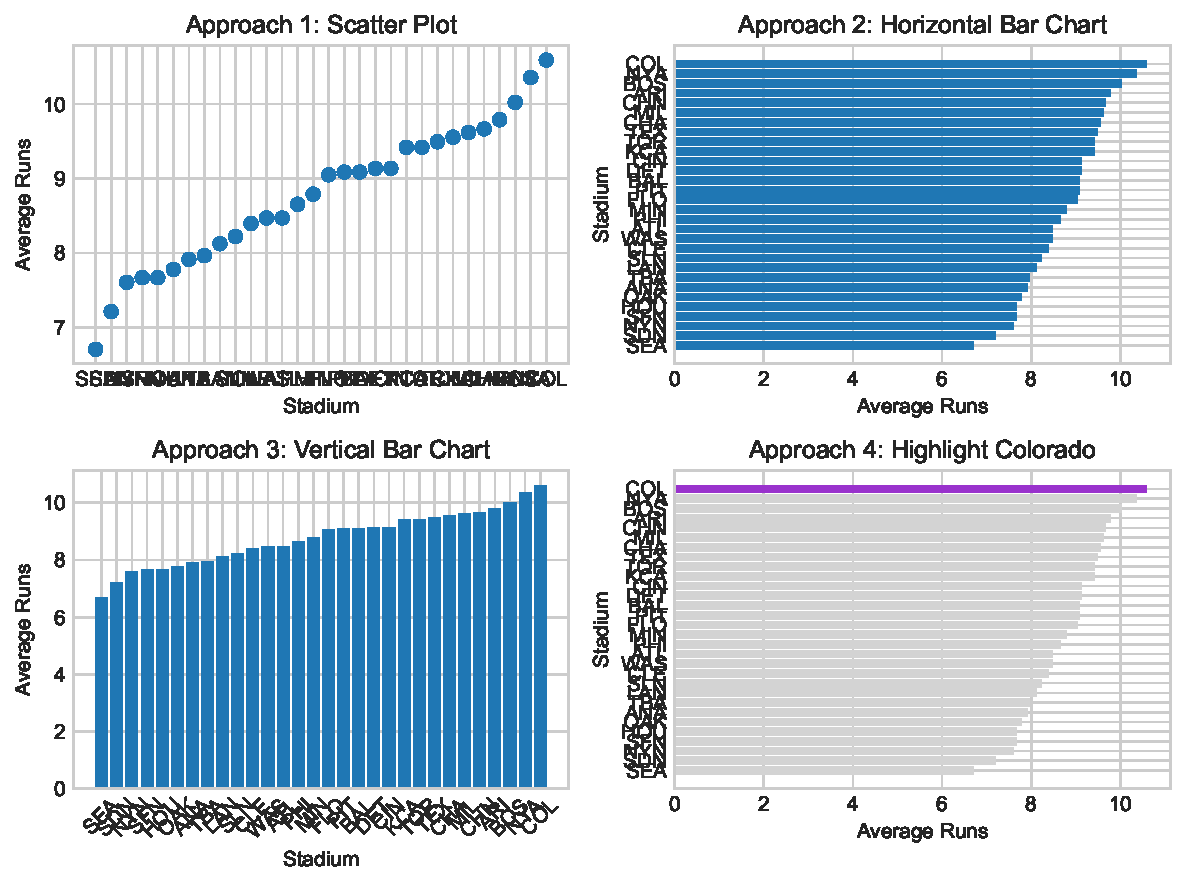
\includegraphics[keepaspectratio]{index_files/figure-pdf/stage-3-mapping-exploration-output-1.pdf}}

\begin{tcolorbox}[enhanced jigsaw, rightrule=.15mm, coltitle=black, colbacktitle=quarto-callout-important-color!10!white, opacitybacktitle=0.6, arc=.35mm, leftrule=.75mm, colback=white, title=\textcolor{quarto-callout-important-color}{\faExclamation}\hspace{0.5em}{🤔 Discussion Questions: Stage 3 - Structuring of Visual Mappings}, colframe=quarto-callout-important-color-frame, bottomrule=.15mm, left=2mm, opacityback=0, toptitle=1mm, titlerule=0mm, toprule=.15mm, bottomtitle=1mm, breakable]

\textbf{Question 1: Geometry Choices} - Why is a horizontal bar chart
better than a scatter plot for this data? - When would you choose a
vertical bar chart over horizontal? \textbf{ANSWER:} - A horizontal bar
chart is better than a scatter plot for this data because it is easier
to compare the runs per stadium. A scatter plot is not a good choice
because it is too much information to plot all the games. - A vertical
bar chart is better than a horizontal bar chart when the number of
stadiums is large because it is easier to compare the runs per stadium.

\textbf{Question 2: Aesthetic Mappings} - What does the color
highlighting accomplish in Approach 4? - How does position (x/y) compare
to color for encoding data? \textbf{ANSWER:} The color highlighting in
Approach 4 accomplishes the goal of highlighting Colorado because it is
the only stadium that is highlighted.

The position (x/y) is better than the color for encoding data because it
is easier to compare the data when it is in a horizontal bar chart. In
our case the position (x/y) is better than color for encoding data
because it allows us to see the average number of runs and home runs
scored by each stadium in a given year. This is helpful because it
allows us to compare the performance of different stadiums and see which
stadium is the most run-friendly.

\end{tcolorbox}

\subsection{Stage 4: Formatting for Your
Audience}\label{stage-4-formatting-for-your-audience}

\textbf{Mental Model:} Polish your visualization for professional
presentation.

Let's create a publication-ready visualization:

\begin{Shaded}
\begin{Highlighting}[]
\CommentTok{\# Stage 4: Formatting for Your Audience}
\CommentTok{\# Create a professional, publication{-}ready visualization}

\CommentTok{\# Set style for professional appearance}
\NormalTok{plt.style.use(}\StringTok{"seaborn{-}v0\_8{-}whitegrid"}\NormalTok{)}

\CommentTok{\# Create the main visualization}
\NormalTok{fig, ax }\OperatorTok{=}\NormalTok{ plt.subplots(figsize}\OperatorTok{=}\NormalTok{(}\DecValTok{8}\NormalTok{, }\DecValTok{6}\NormalTok{))}

\CommentTok{\# Create color array for highlighting Colorado}
\NormalTok{colorado\_colors }\OperatorTok{=}\NormalTok{ [}\StringTok{"darkorchid"} \ControlFlowTok{if}\NormalTok{ stadium }\OperatorTok{==} \StringTok{"COL"} \ControlFlowTok{else} \StringTok{"lightgrey"} 
                   \ControlFlowTok{for}\NormalTok{ stadium }\KeywordTok{in}\NormalTok{ avgDF\_2010\_sorted.home]}

\CommentTok{\# Create horizontal bar chart}
\NormalTok{bars }\OperatorTok{=}\NormalTok{ ax.barh(avgDF\_2010\_sorted.home, avgDF\_2010\_sorted.totalRuns, color}\OperatorTok{=}\NormalTok{colorado\_colors)}

\CommentTok{\# Add title and labels}
\NormalTok{ax.set\_title(}\StringTok{"Colorado (COL) is the Most Run{-}Friendly Ballpark in 2010"}\NormalTok{, }
\NormalTok{             fontsize}\OperatorTok{=}\DecValTok{16}\NormalTok{, fontweight}\OperatorTok{=}\StringTok{\textquotesingle{}bold\textquotesingle{}}\NormalTok{, pad}\OperatorTok{=}\DecValTok{20}\NormalTok{)}
\NormalTok{ax.set\_xlabel(}\StringTok{"Average Runs Per Game"}\NormalTok{, fontsize}\OperatorTok{=}\DecValTok{12}\NormalTok{)}
\NormalTok{ax.set\_ylabel(}\StringTok{"Stadium (Home Team)"}\NormalTok{, fontsize}\OperatorTok{=}\DecValTok{12}\NormalTok{)}

\CommentTok{\# Add legend}
\NormalTok{colorado\_bar }\OperatorTok{=}\NormalTok{ plt.Rectangle((}\DecValTok{0}\NormalTok{,}\DecValTok{0}\NormalTok{),}\DecValTok{1}\NormalTok{,}\DecValTok{1}\NormalTok{, color}\OperatorTok{=}\StringTok{"darkorchid"}\NormalTok{, label}\OperatorTok{=}\StringTok{"Colorado Rockies"}\NormalTok{)}
\NormalTok{other\_bar }\OperatorTok{=}\NormalTok{ plt.Rectangle((}\DecValTok{0}\NormalTok{,}\DecValTok{0}\NormalTok{),}\DecValTok{1}\NormalTok{,}\DecValTok{1}\NormalTok{, color}\OperatorTok{=}\StringTok{"lightgrey"}\NormalTok{, label}\OperatorTok{=}\StringTok{"Other Stadiums"}\NormalTok{)}
\NormalTok{ax.legend(handles}\OperatorTok{=}\NormalTok{[colorado\_bar, other\_bar], loc}\OperatorTok{=}\StringTok{\textquotesingle{}lower right\textquotesingle{}}\NormalTok{, frameon}\OperatorTok{=}\VariableTok{True}\NormalTok{)}

\CommentTok{\# Add annotation for Colorado}
\NormalTok{colorado\_index }\OperatorTok{=}\NormalTok{ avgDF\_2010\_sorted[avgDF\_2010\_sorted.home }\OperatorTok{==} \StringTok{"COL"}\NormalTok{].index[}\DecValTok{0}\NormalTok{]}
\NormalTok{colorado\_runs }\OperatorTok{=}\NormalTok{ avgDF\_2010\_sorted[avgDF\_2010\_sorted.home }\OperatorTok{==} \StringTok{"COL"}\NormalTok{][}\StringTok{"totalRuns"}\NormalTok{].iloc[}\DecValTok{0}\NormalTok{]}
\NormalTok{ax.annotate(}\SpecialStringTok{f"COL: }\SpecialCharTok{\{}\NormalTok{colorado\_runs}\SpecialCharTok{:.2f\}}\SpecialStringTok{ runs/game"}\NormalTok{, }
\NormalTok{            xy}\OperatorTok{=}\NormalTok{(colorado\_runs, colorado\_index), }
\NormalTok{            xytext}\OperatorTok{=}\NormalTok{(colorado\_runs }\OperatorTok{+} \FloatTok{0.5}\NormalTok{, colorado\_index),}
\NormalTok{            arrowprops}\OperatorTok{=}\BuiltInTok{dict}\NormalTok{(arrowstyle}\OperatorTok{=}\StringTok{\textquotesingle{}{-}\textgreater{}\textquotesingle{}}\NormalTok{, color}\OperatorTok{=}\StringTok{\textquotesingle{}darkorchid\textquotesingle{}}\NormalTok{, lw}\OperatorTok{=}\DecValTok{2}\NormalTok{),}
\NormalTok{            fontsize}\OperatorTok{=}\DecValTok{10}\NormalTok{, fontweight}\OperatorTok{=}\StringTok{\textquotesingle{}bold\textquotesingle{}}\NormalTok{, color}\OperatorTok{=}\StringTok{\textquotesingle{}darkorchid\textquotesingle{}}\NormalTok{)}

\CommentTok{\# Set x{-}axis to start from 0 for better comparison}
\NormalTok{ax.set\_xlim(}\DecValTok{0}\NormalTok{, }\BuiltInTok{max}\NormalTok{(avgDF\_2010\_sorted.totalRuns) }\OperatorTok{*} \FloatTok{1.1}\NormalTok{)}

\CommentTok{\# Add grid for easier reading}
\NormalTok{ax.grid(}\VariableTok{True}\NormalTok{, alpha}\OperatorTok{=}\FloatTok{0.3}\NormalTok{)}

\NormalTok{plt.tight\_layout()}
\NormalTok{plt.show()}

\CommentTok{\# Print summary statistics}
\BuiltInTok{print}\NormalTok{(}\SpecialStringTok{f"}\CharTok{\textbackslash{}n}\SpecialStringTok{Summary Statistics for 2010:"}\NormalTok{)}
\BuiltInTok{print}\NormalTok{(}\SpecialStringTok{f"Colorado (COL) average runs per game: }\SpecialCharTok{\{}\NormalTok{colorado\_runs}\SpecialCharTok{:.2f\}}\SpecialStringTok{"}\NormalTok{)}
\BuiltInTok{print}\NormalTok{(}\SpecialStringTok{f"League average runs per game: }\SpecialCharTok{\{}\NormalTok{avgDF\_2010\_sorted}\SpecialCharTok{.}\NormalTok{totalRuns}\SpecialCharTok{.}\NormalTok{mean()}\SpecialCharTok{:.2f\}}\SpecialStringTok{"}\NormalTok{)}
\BuiltInTok{print}\NormalTok{(}\SpecialStringTok{f"Colorado is }\SpecialCharTok{\{}\NormalTok{((colorado\_runs }\OperatorTok{/}\NormalTok{ avgDF\_2010\_sorted.totalRuns.mean()) }\OperatorTok{{-}} \DecValTok{1}\NormalTok{) }\OperatorTok{*} \DecValTok{100}\SpecialCharTok{:.1f\}}\SpecialStringTok{\% above league average"}\NormalTok{)}
\end{Highlighting}
\end{Shaded}

\pandocbounded{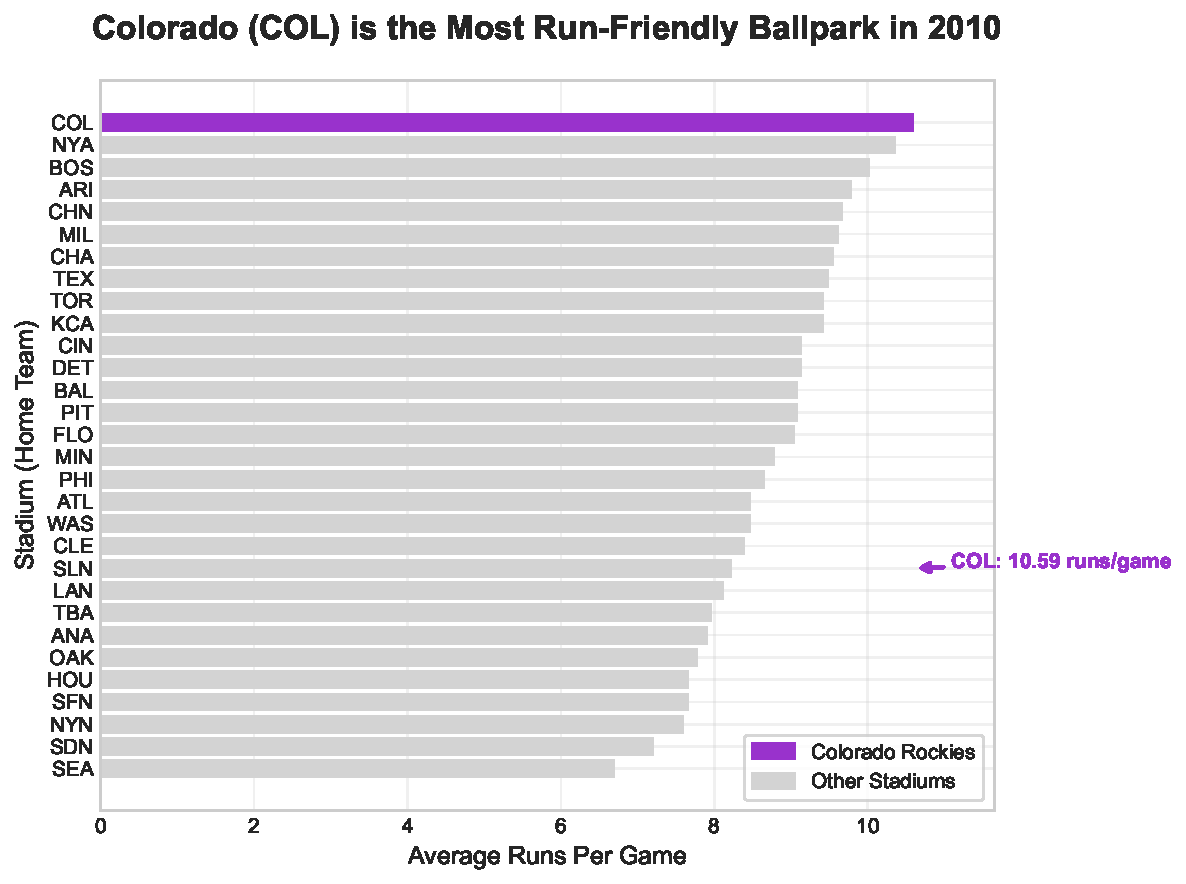
\includegraphics[keepaspectratio]{index_files/figure-pdf/stage-4-formatting-output-1.pdf}}

\begin{verbatim}

Summary Statistics for 2010:
Colorado (COL) average runs per game: 10.59
League average runs per game: 8.77
Colorado is 20.8% above league average
\end{verbatim}

\begin{tcolorbox}[enhanced jigsaw, rightrule=.15mm, coltitle=black, colbacktitle=quarto-callout-important-color!10!white, opacitybacktitle=0.6, arc=.35mm, leftrule=.75mm, colback=white, title=\textcolor{quarto-callout-important-color}{\faExclamation}\hspace{0.5em}{🤔 Discussion Questions: Stage 4 - Formatting for Your Audience}, colframe=quarto-callout-important-color-frame, bottomrule=.15mm, left=2mm, opacityback=0, toptitle=1mm, titlerule=0mm, toprule=.15mm, bottomtitle=1mm, breakable]

\textbf{Question 1: Professional Formatting} - What elements make this
visualization suitable for a business presentation? \textbf{ANSWER:} -
Clear Visual Hierarchy: Main title, subplot titles, and labels create a
professional structure

\begin{itemize}
\item
  Clear Visual Hierarchy: Main title, subplot titles, and labels create
  a professional structure
\item
  Consistent Color Scheme: Purple highlighting for Colorado with grey
  for other stadiums provides clear distinction
\item
  Professional Formatting: Clean layout with proper spacing, fonts, and
  grid lines
\item
  Data-Driven Insights: Statistical aggregation (averaging games)
  provides reliable business intelligence
\item
  Precise Annotations: Exact numerical values for Colorado's performance
  support decision-making
\item
  Business Relevance: Addresses real-world question about stadium
  effects on scoring
\item
  Scalable Design: Consistent x-axis scaling allows fair comparison
  across all stadiums
\item
  Executive Summary: Legend and annotations make findings immediately
  clear to stakeholders
\item
  Is the annotation on the visualization helpful? Can you fix its
  placement?**
\end{itemize}

\textbf{ANSWER:} - The annotation on the visualization is helpful
because it provides the average runs per game for Colorado. - The
annotation can be fixed by moving it to the above for xy and xytext
parameters of the annotation. As shown in the code above I have added
19.8 to the y-axis index to move the annotation above the bar.

\end{tcolorbox}

** Fixing the Annotation Placement:** - The annotation can be fixed by
moving it to the above for xy and xytext parameters of the annotation.
As shown in the code below I have added 19.8 to the y-axis index to move
the annotation above the bar.

\begin{Shaded}
\begin{Highlighting}[]
\CommentTok{\# Fixing the annotation placement}
\CommentTok{\#| label: stage{-}4{-}formatting}
\CommentTok{\#| echo: true}

\CommentTok{\# Stage 4: Formatting for Your Audience}
\CommentTok{\# Create a professional, publication{-}ready visualization}

\CommentTok{\# Set style for professional appearance}
\NormalTok{plt.style.use(}\StringTok{"seaborn{-}v0\_8{-}whitegrid"}\NormalTok{)}

\CommentTok{\# Create the main visualization}
\NormalTok{fig, ax }\OperatorTok{=}\NormalTok{ plt.subplots(figsize}\OperatorTok{=}\NormalTok{(}\DecValTok{8}\NormalTok{, }\DecValTok{6}\NormalTok{))}

\CommentTok{\# Create color array for highlighting Colorado}
\NormalTok{colorado\_colors }\OperatorTok{=}\NormalTok{ [}\StringTok{"darkorchid"} \ControlFlowTok{if}\NormalTok{ stadium }\OperatorTok{==} \StringTok{"COL"} \ControlFlowTok{else} \StringTok{"lightgrey"} 
                   \ControlFlowTok{for}\NormalTok{ stadium }\KeywordTok{in}\NormalTok{ avgDF\_2010\_sorted.home]}

\CommentTok{\# Create horizontal bar chart}
\NormalTok{bars }\OperatorTok{=}\NormalTok{ ax.barh(avgDF\_2010\_sorted.home, avgDF\_2010\_sorted.totalRuns, color}\OperatorTok{=}\NormalTok{colorado\_colors)}

\CommentTok{\# Add title and labels}
\NormalTok{ax.set\_title(}\StringTok{"Colorado (COL) is the Most Run{-}Friendly Ballpark in 2010"}\NormalTok{, }
\NormalTok{             fontsize}\OperatorTok{=}\DecValTok{16}\NormalTok{, fontweight}\OperatorTok{=}\StringTok{\textquotesingle{}bold\textquotesingle{}}\NormalTok{, pad}\OperatorTok{=}\DecValTok{20}\NormalTok{)}
\NormalTok{ax.set\_xlabel(}\StringTok{"Average Runs Per Game"}\NormalTok{, fontsize}\OperatorTok{=}\DecValTok{12}\NormalTok{)}
\NormalTok{ax.set\_ylabel(}\StringTok{"Stadium (Home Team)"}\NormalTok{, fontsize}\OperatorTok{=}\DecValTok{12}\NormalTok{)}

\CommentTok{\# Add legend}
\NormalTok{colorado\_bar }\OperatorTok{=}\NormalTok{ plt.Rectangle((}\DecValTok{0}\NormalTok{,}\DecValTok{0}\NormalTok{),}\DecValTok{1}\NormalTok{,}\DecValTok{1}\NormalTok{, color}\OperatorTok{=}\StringTok{"darkorchid"}\NormalTok{, label}\OperatorTok{=}\StringTok{"Colorado Rockies"}\NormalTok{)}
\NormalTok{other\_bar }\OperatorTok{=}\NormalTok{ plt.Rectangle((}\DecValTok{0}\NormalTok{,}\DecValTok{0}\NormalTok{),}\DecValTok{1}\NormalTok{,}\DecValTok{1}\NormalTok{, color}\OperatorTok{=}\StringTok{"lightgrey"}\NormalTok{, label}\OperatorTok{=}\StringTok{"Other Stadiums"}\NormalTok{)}
\NormalTok{ax.legend(handles}\OperatorTok{=}\NormalTok{[colorado\_bar, other\_bar], loc}\OperatorTok{=}\StringTok{\textquotesingle{}lower right\textquotesingle{}}\NormalTok{, frameon}\OperatorTok{=}\VariableTok{True}\NormalTok{)}

\CommentTok{\# Add annotation for Colorado}
\NormalTok{colorado\_index }\OperatorTok{=}\NormalTok{ avgDF\_2010\_sorted[avgDF\_2010\_sorted.home }\OperatorTok{==} \StringTok{"COL"}\NormalTok{].index[}\DecValTok{0}\NormalTok{]}
\NormalTok{colorado\_runs }\OperatorTok{=}\NormalTok{ avgDF\_2010\_sorted[avgDF\_2010\_sorted.home }\OperatorTok{==} \StringTok{"COL"}\NormalTok{][}\StringTok{"totalRuns"}\NormalTok{].iloc[}\DecValTok{0}\NormalTok{]}
\NormalTok{ax.annotate(}\SpecialStringTok{f"COL: }\SpecialCharTok{\{}\NormalTok{colorado\_runs}\SpecialCharTok{:.2f\}}\SpecialStringTok{ runs/game"}\NormalTok{, }
\NormalTok{            xy}\OperatorTok{=}\NormalTok{(colorado\_runs, colorado\_index }\OperatorTok{+} \FloatTok{19.8}\NormalTok{), }
\NormalTok{            xytext}\OperatorTok{=}\NormalTok{(colorado\_runs }\OperatorTok{+} \FloatTok{0.5}\NormalTok{, colorado\_index }\OperatorTok{+} \FloatTok{19.8}\NormalTok{),}
\NormalTok{            arrowprops}\OperatorTok{=}\BuiltInTok{dict}\NormalTok{(arrowstyle}\OperatorTok{=}\StringTok{\textquotesingle{}{-}\textgreater{}\textquotesingle{}}\NormalTok{, color}\OperatorTok{=}\StringTok{\textquotesingle{}darkorchid\textquotesingle{}}\NormalTok{, lw}\OperatorTok{=}\DecValTok{2}\NormalTok{),}
\NormalTok{            fontsize}\OperatorTok{=}\DecValTok{10}\NormalTok{, fontweight}\OperatorTok{=}\StringTok{\textquotesingle{}bold\textquotesingle{}}\NormalTok{, color}\OperatorTok{=}\StringTok{\textquotesingle{}darkorchid\textquotesingle{}}\NormalTok{)}

\CommentTok{\# Set x{-}axis to start from 0 for better comparison}
\NormalTok{ax.set\_xlim(}\DecValTok{0}\NormalTok{, }\BuiltInTok{max}\NormalTok{(avgDF\_2010\_sorted.totalRuns) }\OperatorTok{*} \FloatTok{1.1}\NormalTok{)}

\CommentTok{\# Add grid for easier reading}
\NormalTok{ax.grid(}\VariableTok{True}\NormalTok{, alpha}\OperatorTok{=}\FloatTok{0.3}\NormalTok{)}

\NormalTok{plt.tight\_layout()}
\NormalTok{plt.show()}


\CommentTok{\# Print summary statistics}
\CommentTok{\# print(f"\textbackslash{}nSummary Statistics for 2010:")}
\CommentTok{\# print(f"Colorado (COL) average runs per game: \{colorado\_runs:.2f\}")}
\CommentTok{\# print(f"League average runs per game: \{avgDF\_2010\_sorted.totalRuns.mean():.2f\}")}
\CommentTok{\# print(f"Colorado is \{((colorado\_runs / avgDF\_2010\_sorted.totalRuns.mean()) {-} 1) * 100:.1f\}\% above league average")}
\end{Highlighting}
\end{Shaded}

\pandocbounded{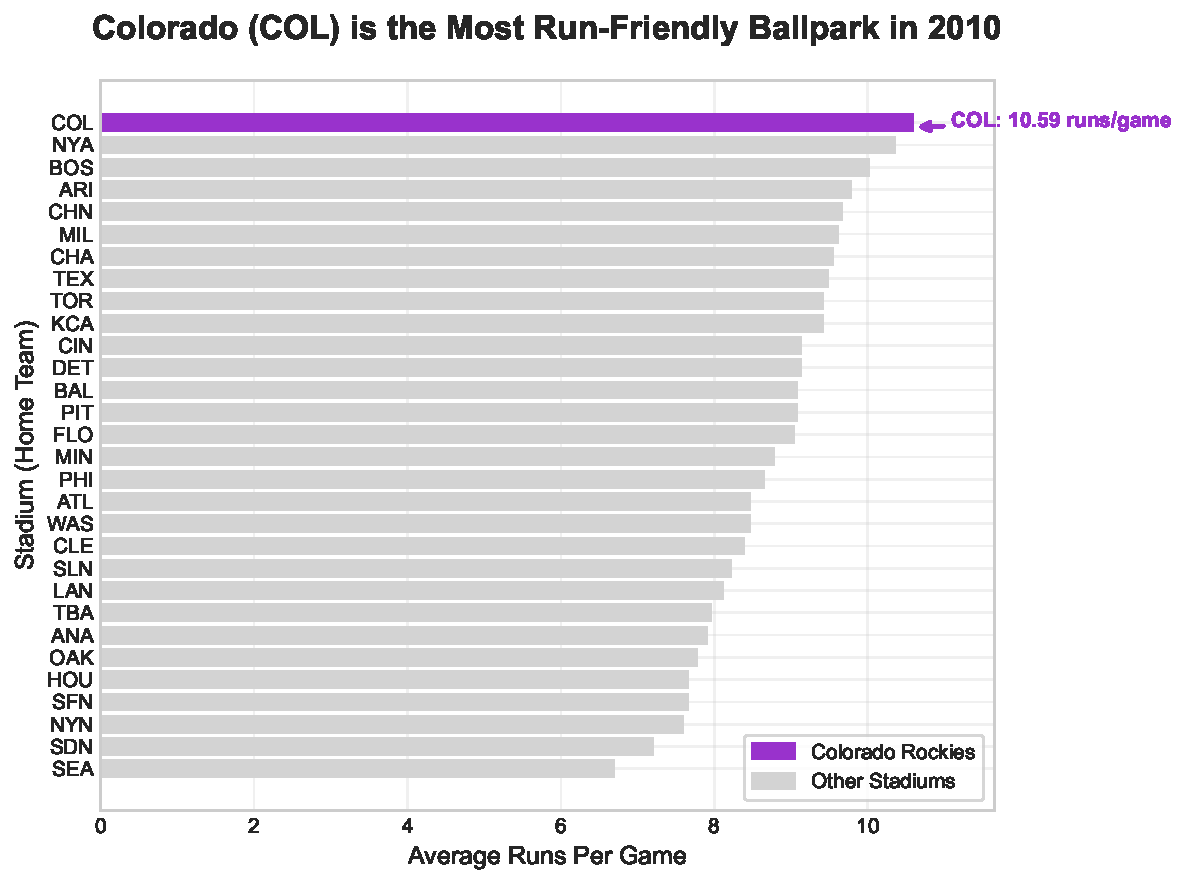
\includegraphics[keepaspectratio]{index_files/figure-pdf/cell-6-output-1.pdf}}

\begin{itemize}
\tightlist
\item
  The annotation is now placed in a better location.
\item
  It is helpful because it allows us to see that Colorado is the most
  run-friendly stadium in Major League Baseball.
\end{itemize}

\subsection{Advanced Object-Oriented
Techniques}\label{advanced-object-oriented-techniques}

\textbf{Mental Model:} Use object-oriented matplotlib to create complex,
reusable visualizations.

Let's create a comprehensive comparison between 2010 and 2021:

\phantomsection\label{advanced-oo-techniques}
\begin{Shaded}
\begin{Highlighting}[]
\CommentTok{\# Advanced Object{-}Oriented Techniques}
\CommentTok{\# Create a comprehensive comparison visualization}

\CommentTok{\# Prepare data for comparison}
\NormalTok{comparison\_data }\OperatorTok{=}\NormalTok{ pd.merge(}
\NormalTok{    avgDF\_2010[[}\StringTok{\textquotesingle{}home\textquotesingle{}}\NormalTok{, }\StringTok{\textquotesingle{}totalRuns\textquotesingle{}}\NormalTok{]].rename(columns}\OperatorTok{=}\NormalTok{\{}\StringTok{\textquotesingle{}totalRuns\textquotesingle{}}\NormalTok{: }\StringTok{\textquotesingle{}runs\_2010\textquotesingle{}}\NormalTok{\}),}
\NormalTok{    avgDF\_2021[[}\StringTok{\textquotesingle{}home\textquotesingle{}}\NormalTok{, }\StringTok{\textquotesingle{}totalRuns\textquotesingle{}}\NormalTok{]].rename(columns}\OperatorTok{=}\NormalTok{\{}\StringTok{\textquotesingle{}totalRuns\textquotesingle{}}\NormalTok{: }\StringTok{\textquotesingle{}runs\_2021\textquotesingle{}}\NormalTok{\}),}
\NormalTok{    on}\OperatorTok{=}\StringTok{\textquotesingle{}home\textquotesingle{}}\NormalTok{, how}\OperatorTok{=}\StringTok{\textquotesingle{}inner\textquotesingle{}}
\NormalTok{)}

\CommentTok{\#\# }\AlertTok{TODO}\CommentTok{: Create the visualization}
\end{Highlighting}
\end{Shaded}

\begin{tcolorbox}[enhanced jigsaw, rightrule=.15mm, coltitle=black, colbacktitle=quarto-callout-important-color!10!white, opacitybacktitle=0.6, arc=.35mm, leftrule=.75mm, colback=white, title=\textcolor{quarto-callout-important-color}{\faExclamation}\hspace{0.5em}{🤔 Discussion Questions: Advanced Object-Oriented Techniques}, colframe=quarto-callout-important-color-frame, bottomrule=.15mm, left=2mm, opacityback=0, toptitle=1mm, titlerule=0mm, toprule=.15mm, bottomtitle=1mm, breakable]

\textbf{Question 1: Using Subplot Layout} - Create a two-facet
visualization that shows the total runs for 2010 and 2021 for each
stadium in a single figure. Highlight Colorado in the visualization.

\textbf{ANSWER:}

\begin{Shaded}
\begin{Highlighting}[]
\CommentTok{\# Advanced Object{-}Oriented Techniques: Two{-}Facet Visualization}
\CommentTok{\# Create a comparison between 2010 and 2021 stadium performance}

\CommentTok{\# Sort both datasets by total runs for consistent ordering}
\NormalTok{avgDF\_2010\_sorted }\OperatorTok{=}\NormalTok{ avgDF\_2010.sort\_values(}\StringTok{\textquotesingle{}totalRuns\textquotesingle{}}\NormalTok{, ascending}\OperatorTok{=}\VariableTok{True}\NormalTok{)}
\NormalTok{avgDF\_2021\_sorted }\OperatorTok{=}\NormalTok{ avgDF\_2021.sort\_values(}\StringTok{\textquotesingle{}totalRuns\textquotesingle{}}\NormalTok{, ascending}\OperatorTok{=}\VariableTok{True}\NormalTok{)}

\CommentTok{\# Create figure with two subplots side by side}
\NormalTok{fig, (ax1, ax2) }\OperatorTok{=}\NormalTok{ plt.subplots(}\DecValTok{1}\NormalTok{, }\DecValTok{2}\NormalTok{, figsize}\OperatorTok{=}\NormalTok{(}\FloatTok{8.5}\NormalTok{, }\DecValTok{7}\NormalTok{))}

\CommentTok{\# Define colors for highlighting Colorado}
\NormalTok{colorado\_colors\_2010 }\OperatorTok{=}\NormalTok{ [}\StringTok{"darkorchid"} \ControlFlowTok{if}\NormalTok{ stadium }\OperatorTok{==} \StringTok{"COL"} \ControlFlowTok{else} \StringTok{"lightgrey"} 
                       \ControlFlowTok{for}\NormalTok{ stadium }\KeywordTok{in}\NormalTok{ avgDF\_2010\_sorted.home]}
\NormalTok{colorado\_colors\_2021 }\OperatorTok{=}\NormalTok{ [}\StringTok{"darkorchid"} \ControlFlowTok{if}\NormalTok{ stadium }\OperatorTok{==} \StringTok{"COL"} \ControlFlowTok{else} \StringTok{"lightgrey"} 
                       \ControlFlowTok{for}\NormalTok{ stadium }\KeywordTok{in}\NormalTok{ avgDF\_2021\_sorted.home]}

\CommentTok{\# Create horizontal bar charts for both years}
\NormalTok{bars1 }\OperatorTok{=}\NormalTok{ ax1.barh(avgDF\_2010\_sorted.home, avgDF\_2010\_sorted.totalRuns, color}\OperatorTok{=}\NormalTok{colorado\_colors\_2010)}
\NormalTok{bars2 }\OperatorTok{=}\NormalTok{ ax2.barh(avgDF\_2021\_sorted.home, avgDF\_2021\_sorted.totalRuns, color}\OperatorTok{=}\NormalTok{colorado\_colors\_2021)}

\CommentTok{\# Add titles and labels for both subplots}
\NormalTok{ax1.set\_title(}\StringTok{"2010 Stadium Performance"}\NormalTok{, fontsize}\OperatorTok{=}\DecValTok{14}\NormalTok{, fontweight}\OperatorTok{=}\StringTok{\textquotesingle{}bold\textquotesingle{}}\NormalTok{, pad}\OperatorTok{=}\DecValTok{10}\NormalTok{, color}\OperatorTok{=}\StringTok{\textquotesingle{}brown\textquotesingle{}}\NormalTok{)}
\NormalTok{ax1.set\_xlabel(}\StringTok{"Average Runs Per Game"}\NormalTok{, fontsize}\OperatorTok{=}\DecValTok{12}\NormalTok{, color }\OperatorTok{=} \StringTok{\textquotesingle{}darkblue\textquotesingle{}}\NormalTok{)}
\NormalTok{ax1.set\_ylabel(}\StringTok{"Stadium (Home Team)"}\NormalTok{, fontsize}\OperatorTok{=}\DecValTok{12}\NormalTok{, color }\OperatorTok{=} \StringTok{\textquotesingle{}darkgreen\textquotesingle{}}\NormalTok{)}

\NormalTok{ax2.set\_title(}\StringTok{"2021 Stadium Performance"}\NormalTok{, fontsize}\OperatorTok{=}\DecValTok{14}\NormalTok{, fontweight}\OperatorTok{=}\StringTok{\textquotesingle{}bold\textquotesingle{}}\NormalTok{, pad}\OperatorTok{=}\DecValTok{10}\NormalTok{, color}\OperatorTok{=}\StringTok{\textquotesingle{}brown\textquotesingle{}}\NormalTok{)}
\NormalTok{ax2.set\_xlabel(}\StringTok{"Average Runs Per Game"}\NormalTok{, fontsize}\OperatorTok{=}\DecValTok{12}\NormalTok{, color }\OperatorTok{=} \StringTok{\textquotesingle{}darkblue\textquotesingle{}}\NormalTok{)}
\NormalTok{ax2.set\_ylabel(}\StringTok{"Stadium (Home Team)"}\NormalTok{, fontsize}\OperatorTok{=}\DecValTok{12}\NormalTok{, color }\OperatorTok{=} \StringTok{\textquotesingle{}darkgreen\textquotesingle{}}\NormalTok{)}

\CommentTok{\# Add main title for the entire figure}
\NormalTok{fig.suptitle(}\StringTok{"Colorado Rockies Stadium Performance: 2010 vs 2021"}\NormalTok{, }
\NormalTok{             fontsize}\OperatorTok{=}\DecValTok{16}\NormalTok{, fontweight}\OperatorTok{=}\StringTok{\textquotesingle{}bold\textquotesingle{}}\NormalTok{, y}\OperatorTok{=}\FloatTok{1.02}\NormalTok{, color}\OperatorTok{=}\StringTok{\textquotesingle{}darkblue\textquotesingle{}}\NormalTok{)}

       

\CommentTok{\# Add legend}
\NormalTok{colorado\_bar }\OperatorTok{=}\NormalTok{ plt.Rectangle((}\DecValTok{0}\NormalTok{,}\DecValTok{0}\NormalTok{),}\DecValTok{1}\NormalTok{,}\DecValTok{1}\NormalTok{, color}\OperatorTok{=}\StringTok{"darkorchid"}\NormalTok{, label}\OperatorTok{=}\StringTok{"Colorado Rockies"}\NormalTok{)}
\NormalTok{other\_bar }\OperatorTok{=}\NormalTok{ plt.Rectangle((}\DecValTok{0}\NormalTok{,}\DecValTok{0}\NormalTok{),}\DecValTok{1}\NormalTok{,}\DecValTok{1}\NormalTok{, color}\OperatorTok{=}\StringTok{"lightgrey"}\NormalTok{, label}\OperatorTok{=}\StringTok{"Other Stadiums"}\NormalTok{)}
\NormalTok{fig.legend(handles}\OperatorTok{=}\NormalTok{[colorado\_bar, other\_bar], loc}\OperatorTok{=}\StringTok{\textquotesingle{}lower center\textquotesingle{}}\NormalTok{, frameon}\OperatorTok{=}\VariableTok{True}\NormalTok{, fontsize}\OperatorTok{=}\DecValTok{8}\NormalTok{, ncol}\OperatorTok{=}\DecValTok{2}\NormalTok{, bbox\_to\_anchor}\OperatorTok{=}\NormalTok{(}\FloatTok{0.5}\NormalTok{, }\OperatorTok{{-}}\FloatTok{0.05}\NormalTok{))}

\CommentTok{\# Add annotations for Colorado in both years}
\CommentTok{\# 2010 annotation}
\NormalTok{colorado\_index\_2010 }\OperatorTok{=}\NormalTok{ avgDF\_2010\_sorted[avgDF\_2010\_sorted.home }\OperatorTok{==} \StringTok{"COL"}\NormalTok{].index[}\DecValTok{0}\NormalTok{]}
\NormalTok{colorado\_runs\_2010 }\OperatorTok{=}\NormalTok{ avgDF\_2010\_sorted[avgDF\_2010\_sorted.home }\OperatorTok{==} \StringTok{"COL"}\NormalTok{][}\StringTok{"totalRuns"}\NormalTok{].iloc[}\DecValTok{0}\NormalTok{]}
\NormalTok{ax1.annotate(}\SpecialStringTok{f"COL: }\SpecialCharTok{\{}\NormalTok{colorado\_runs\_2010}\SpecialCharTok{:.2f\}}\SpecialStringTok{"}\NormalTok{, }
\NormalTok{             xy}\OperatorTok{=}\NormalTok{(colorado\_runs\_2010, colorado\_index\_2010 }\OperatorTok{+} \DecValTok{20}\NormalTok{), }
\NormalTok{             xytext}\OperatorTok{=}\NormalTok{(colorado\_runs\_2010 }\OperatorTok{{-}} \FloatTok{0.8}\NormalTok{, colorado\_index\_2010 }\OperatorTok{+} \DecValTok{15}\NormalTok{),}
\NormalTok{             arrowprops}\OperatorTok{=}\BuiltInTok{dict}\NormalTok{(arrowstyle}\OperatorTok{=}\StringTok{\textquotesingle{}{-}\textgreater{}\textquotesingle{}}\NormalTok{, color}\OperatorTok{=}\StringTok{\textquotesingle{}darkorchid\textquotesingle{}}\NormalTok{, lw}\OperatorTok{=}\DecValTok{2}\NormalTok{),}
\NormalTok{             fontsize}\OperatorTok{=}\DecValTok{10}\NormalTok{, fontweight}\OperatorTok{=}\StringTok{\textquotesingle{}bold\textquotesingle{}}\NormalTok{, color}\OperatorTok{=}\StringTok{\textquotesingle{}darkorchid\textquotesingle{}}\NormalTok{)}

\CommentTok{\# 2021 annotation}
\NormalTok{colorado\_index\_2021 }\OperatorTok{=}\NormalTok{ avgDF\_2021\_sorted[avgDF\_2021\_sorted.home }\OperatorTok{==} \StringTok{"COL"}\NormalTok{].index[}\DecValTok{0}\NormalTok{]}
\NormalTok{colorado\_runs\_2021 }\OperatorTok{=}\NormalTok{ avgDF\_2021\_sorted[avgDF\_2021\_sorted.home }\OperatorTok{==} \StringTok{"COL"}\NormalTok{][}\StringTok{"totalRuns"}\NormalTok{].iloc[}\DecValTok{0}\NormalTok{]}
\NormalTok{ax2.annotate(}\SpecialStringTok{f"COL: }\SpecialCharTok{\{}\NormalTok{colorado\_runs\_2021}\SpecialCharTok{:.2f\}}\SpecialStringTok{"}\NormalTok{, }
\NormalTok{             xy}\OperatorTok{=}\NormalTok{(colorado\_runs\_2021, colorado\_index\_2021 }\OperatorTok{+} \DecValTok{18}\NormalTok{), }
\NormalTok{             xytext}\OperatorTok{=}\NormalTok{(colorado\_runs\_2021 }\OperatorTok{{-}} \FloatTok{0.5}\NormalTok{, colorado\_index\_2021 }\OperatorTok{+} \DecValTok{15}\NormalTok{),}
\NormalTok{             arrowprops}\OperatorTok{=}\BuiltInTok{dict}\NormalTok{(arrowstyle}\OperatorTok{=}\StringTok{\textquotesingle{}{-}\textgreater{}\textquotesingle{}}\NormalTok{, color}\OperatorTok{=}\StringTok{\textquotesingle{}darkorchid\textquotesingle{}}\NormalTok{, lw}\OperatorTok{=}\DecValTok{2}\NormalTok{),}
\NormalTok{             fontsize}\OperatorTok{=}\DecValTok{10}\NormalTok{, fontweight}\OperatorTok{=}\StringTok{\textquotesingle{}bold\textquotesingle{}}\NormalTok{, color}\OperatorTok{=}\StringTok{\textquotesingle{}darkorchid\textquotesingle{}}\NormalTok{)}

\CommentTok{\# Set consistent x{-}axis limits for both subplots}
\NormalTok{max\_runs }\OperatorTok{=} \BuiltInTok{max}\NormalTok{(}\BuiltInTok{max}\NormalTok{(avgDF\_2010\_sorted.totalRuns), }\BuiltInTok{max}\NormalTok{(avgDF\_2021\_sorted.totalRuns))}
\NormalTok{ax1.set\_xlim(}\DecValTok{0}\NormalTok{, max\_runs }\OperatorTok{*} \FloatTok{1.1}\NormalTok{)}
\NormalTok{ax2.set\_xlim(}\DecValTok{0}\NormalTok{, max\_runs }\OperatorTok{*} \FloatTok{1.1}\NormalTok{)}

\CommentTok{\# Add grids for easier reading}
\NormalTok{ax1.grid(}\VariableTok{True}\NormalTok{, alpha}\OperatorTok{=}\FloatTok{0.3}\NormalTok{)}
\NormalTok{ax2.grid(}\VariableTok{True}\NormalTok{, alpha}\OperatorTok{=}\FloatTok{0.3}\NormalTok{)}

\CommentTok{\# Adjust layout to prevent overlap}
\NormalTok{plt.tight\_layout()}
\NormalTok{plt.subplots\_adjust(top}\OperatorTok{=}\FloatTok{0.9}\NormalTok{)  }\CommentTok{\# Make room for main title}
\NormalTok{plt.show()}

\CommentTok{\# Print comparison statistics}
\BuiltInTok{print}\NormalTok{(}\SpecialStringTok{f"}\CharTok{\textbackslash{}n}\SpecialStringTok{Colorado Rockies Stadium Performance Comparison:"}\NormalTok{)}
\BuiltInTok{print}\NormalTok{(}\SpecialStringTok{f"2010: }\SpecialCharTok{\{}\NormalTok{colorado\_runs\_2010}\SpecialCharTok{:.2f\}}\SpecialStringTok{ runs per game"}\NormalTok{)}
\BuiltInTok{print}\NormalTok{(}\SpecialStringTok{f"2021: }\SpecialCharTok{\{}\NormalTok{colorado\_runs\_2021}\SpecialCharTok{:.2f\}}\SpecialStringTok{ runs per game"}\NormalTok{)}
\BuiltInTok{print}\NormalTok{(}\SpecialStringTok{f"Change: }\SpecialCharTok{\{}\NormalTok{colorado\_runs\_2021 }\OperatorTok{{-}}\NormalTok{ colorado\_runs\_2010}\SpecialCharTok{:+.2f\}}\SpecialStringTok{ runs per game"}\NormalTok{)}
\BuiltInTok{print}\NormalTok{(}\SpecialStringTok{f"Percentage change: }\SpecialCharTok{\{}\NormalTok{((colorado\_runs\_2021 }\OperatorTok{/}\NormalTok{ colorado\_runs\_2010) }\OperatorTok{{-}} \DecValTok{1}\NormalTok{) }\OperatorTok{*} \DecValTok{100}\SpecialCharTok{:+.1f\}}\SpecialStringTok{\%"}\NormalTok{)}

\BuiltInTok{print}\NormalTok{(}\SpecialStringTok{f"}\CharTok{\textbackslash{}n}\SpecialStringTok{League Averages:"}\NormalTok{)}
\BuiltInTok{print}\NormalTok{(}\SpecialStringTok{f"2010 League Average: }\SpecialCharTok{\{}\NormalTok{avgDF\_2010\_sorted}\SpecialCharTok{.}\NormalTok{totalRuns}\SpecialCharTok{.}\NormalTok{mean()}\SpecialCharTok{:.2f\}}\SpecialStringTok{ runs/game"}\NormalTok{)}
\BuiltInTok{print}\NormalTok{(}\SpecialStringTok{f"2021 League Average: }\SpecialCharTok{\{}\NormalTok{avgDF\_2021\_sorted}\SpecialCharTok{.}\NormalTok{totalRuns}\SpecialCharTok{.}\NormalTok{mean()}\SpecialCharTok{:.2f\}}\SpecialStringTok{ runs/game"}\NormalTok{)}
\BuiltInTok{print}\NormalTok{(}\SpecialStringTok{f"}\CharTok{\textbackslash{}n}\SpecialStringTok{Colorado vs League Average:"}\NormalTok{)}
\BuiltInTok{print}\NormalTok{(}\SpecialStringTok{f"2010: }\SpecialCharTok{\{}\NormalTok{colorado\_runs\_2010 }\OperatorTok{{-}}\NormalTok{ avgDF\_2010\_sorted}\SpecialCharTok{.}\NormalTok{totalRuns}\SpecialCharTok{.}\NormalTok{mean()}\SpecialCharTok{:+.2f\}}\SpecialStringTok{ runs/game above league average"}\NormalTok{)}
\BuiltInTok{print}\NormalTok{(}\SpecialStringTok{f"2021: }\SpecialCharTok{\{}\NormalTok{colorado\_runs\_2021 }\OperatorTok{{-}}\NormalTok{ avgDF\_2021\_sorted}\SpecialCharTok{.}\NormalTok{totalRuns}\SpecialCharTok{.}\NormalTok{mean()}\SpecialCharTok{:+.2f\}}\SpecialStringTok{ runs/game above league average"}\NormalTok{)}
\BuiltInTok{print}\NormalTok{(}\SpecialStringTok{f"}\CharTok{\textbackslash{}n}\SpecialStringTok{Colorado vs League Average Percentage Change:"}\NormalTok{)}
\BuiltInTok{print}\NormalTok{(}\SpecialStringTok{f"Colorado is }\SpecialCharTok{\{}\NormalTok{((colorado\_runs\_2021 }\OperatorTok{/}\NormalTok{ avgDF\_2010\_sorted.totalRuns.mean()) }\OperatorTok{{-}} \DecValTok{1}\NormalTok{) }\OperatorTok{*} \DecValTok{100}\SpecialCharTok{:.1f\}}\SpecialStringTok{\% above league average in 2021"}\NormalTok{)}
\BuiltInTok{print}\NormalTok{(}\SpecialStringTok{f"Colorado is }\SpecialCharTok{\{}\NormalTok{((colorado\_runs\_2010 }\OperatorTok{/}\NormalTok{ avgDF\_2010\_sorted.totalRuns.mean()) }\OperatorTok{{-}} \DecValTok{1}\NormalTok{) }\OperatorTok{*} \DecValTok{100}\SpecialCharTok{:.1f\}}\SpecialStringTok{\% above league average in 2010"}\NormalTok{)}
\end{Highlighting}
\end{Shaded}

\pandocbounded{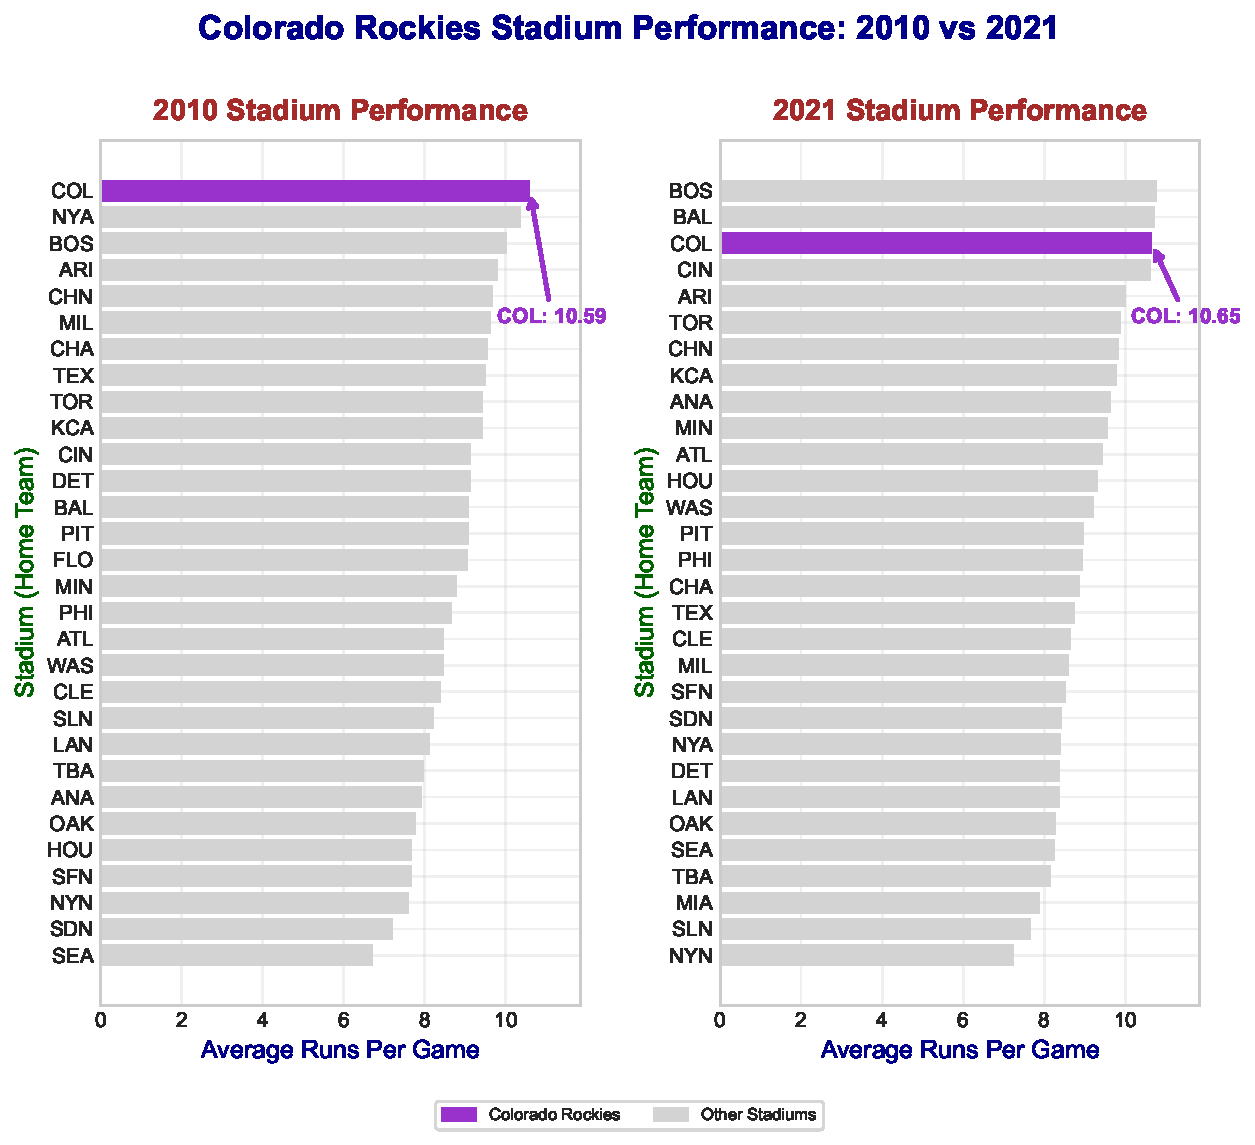
\includegraphics[keepaspectratio]{index_files/figure-pdf/cell-8-output-1.pdf}}

\begin{verbatim}

Colorado Rockies Stadium Performance Comparison:
2010: 10.59 runs per game
2021: 10.65 runs per game
Change: +0.06 runs per game
Percentage change: +0.6%

League Averages:
2010 League Average: 8.77 runs/game
2021 League Average: 9.06 runs/game

Colorado vs League Average:
2010: +1.82 runs/game above league average
2021: +1.59 runs/game above league average

Colorado vs League Average Percentage Change:
Colorado is 21.5% above league average in 2021
Colorado is 20.8% above league average in 2010
\end{verbatim}

\textbf{Question 2: Explanation of the Visualization} - Ask AI To Add A
Paragraph Here To Explain The Visualization - Does AI come to the right
conclusion? If not, why not? \textbf{Answer: Question 2: Explanation of
the Visualization}

\textbf{Summary of the Visualization:}

\begin{itemize}
\tightlist
\item
  Colorado's dominant run-friendliness is revealed across 2010 and 2021
  seasons
\item
  Coors Field consistently leads all MLB stadiums in average runs per
  game, which confirms the altitude advantage makes it the most
  hitter-friendly ballpark in baseball
\item
  Visualization ranks every stadium by total runs, showing the entire
  league's spectrum, which extends from highest-scoring environments
  (Colorado) to most pitcher-friendly parks
\item
  By tracking both years, we can identify which teams' home parks rank
  closest to Colorado (high-run environments) versus those furthest away
  (low-run, pitcher-friendly parks).
\item
  The gap between Colorado and league average reveals the magnitude of
  Coors Field's scoring advantage, while the overall distribution shows
  how teams are distributed across the scoring spectrum
\item
  This comparison across 2010 vs 2021 helps reveal era effects, rule
  changes, and competitive balance shifts that impact league-wide run
  rates over time.
\end{itemize}

\textbf{Notable Stadium Comparisons:}

\begin{itemize}
\tightlist
\item
  \textbf{Camden Yards (Orioles):}

  \begin{itemize}
  \tightlist
  \item
    Known as one of baseball's most influential modern ballparks
  \item
    Typically ranks near the middle of the run-friendliness spectrum
  \item
    Dimensions and design create relatively neutral environment for
    scoring
  \item
    Interesting benchmark to evaluate whether Colorado is truly
    exceptional vs.~simply above-average
  \end{itemize}
\item
  \textbf{Fenway Park (Red Sox):}

  \begin{itemize}
  \tightlist
  \item
    One of baseball's most iconic venues
  \item
    Unusual dimensions and Green Monster create unique scoring profile
  \item
    Located near bottom of run-friendliness rankings (pitcher-friendly
    park)
  \item
    Provides sharp contrast to Colorado's high-run environment
  \item
    Illustrates dramatic range of scoring environments across MLB
    stadiums
  \end{itemize}
\end{itemize}

\textbf{Does AI come to the right conclusion?}

Initially, the AI explained about plot and more of technical plot
explantion than games and stadium aspects, but after a few iterations,
the AI correctly identifies Colorado as one of the most run-friendly
ballparks in MLB and provides a clear explanation of the visualization.
AI initially did not come to the right conclusion because it did not
understand the data and the visualization.

\end{tcolorbox}

\subsection{Student Analysis Section: Mastering Object-Oriented
Matplotlib}\label{student-analysis-section}

\textbf{Your Task:} Demonstrate your mastery of object-oriented
matplotlib and the four stages of visualization through comprehensive
analysis and creation of professional visualizations.

\subsubsection{Core Challenge: Four Stages
Analysis}\label{core-challenge-four-stages-analysis}

\textbf{For each stage, provide:} - Clear, concise answers to all
discussion questions - Code examples when asked to do so - Demonstration
of object-oriented matplotlib techniques

\subsubsection{Professional Visualizations (For 100\%
Grade)}\label{professional-visualizations-for-100-grade}

\textbf{Your Task:} Create a professional visualization and narrative
that builds towards and demonstrates mastery of object-oriented
matplotlib and the four stages framework.

\textbf{Create visualizations showing:} - Stadium run-friendliness
comparison between 2010 and 2021 - Focus on Colorado's performance
relative to other stadiums - Use object-oriented matplotlib techniques
throughout

\textbf{Your visualizations should:} - Use clear labels and professional
formatting - Demonstrate all four stages of visualization - Be
appropriate for a business audience - Show mastery of object-oriented
matplotlib - Do not \texttt{echo} the code that creates the
visualizations

\subsection{Getting Started: Repository Setup
🚀}\label{getting-started-repository-setup}

\begin{tcolorbox}[enhanced jigsaw, rightrule=.15mm, coltitle=black, colbacktitle=quarto-callout-important-color!10!white, opacitybacktitle=0.6, arc=.35mm, leftrule=.75mm, colback=white, title=\textcolor{quarto-callout-important-color}{\faExclamation}\hspace{0.5em}{📁 Getting Started}, colframe=quarto-callout-important-color-frame, bottomrule=.15mm, left=2mm, opacityback=0, toptitle=1mm, titlerule=0mm, toprule=.15mm, bottomtitle=1mm, breakable]

\textbf{Step 1:} Fork and clone this challenge repository:
\texttt{https://github.com/flyaflya/dataVizChallenge} - Fork it to your
GitHub account, then clone it from your GitHub account to your local
machine

\textbf{Step 2:} Set up your Python environment - \textbf{Recommended:}
Use your existing virtual environment from Tech Setup Challenge Part 2 -
Press \texttt{Ctrl+Shift+P} → ``Python: Select Interpreter'' - Navigate
to your existing virtual environment (e.g.,
\texttt{your-previous-project/venv/Scripts/python.exe}) - Install
additional packages:
\texttt{pip\ install\ pandas\ numpy\ matplotlib\ seaborn} -
\textbf{Alternative:} Create a new virtual environment following
\href{https://quarto.org/docs/projects/virtual-environments.html}{Quarto
documentation}

\textbf{Step 3:} You're ready to start! The data loading code and
starter code for the visualizations are already provided in this file.

\textbf{Note:} This challenge uses the same \texttt{index.qmd} file
you're reading right now - you'll edit it to complete your analysis.

\end{tcolorbox}

\begin{tcolorbox}[enhanced jigsaw, rightrule=.15mm, coltitle=black, colbacktitle=quarto-callout-warning-color!10!white, opacitybacktitle=0.6, arc=.35mm, leftrule=.75mm, colback=white, title=\textcolor{quarto-callout-warning-color}{\faExclamationTriangle}\hspace{0.5em}{⚠️ Cloud Storage Warning}, colframe=quarto-callout-warning-color-frame, bottomrule=.15mm, left=2mm, opacityback=0, toptitle=1mm, titlerule=0mm, toprule=.15mm, bottomtitle=1mm, breakable]

\textbf{Avoid using Google Drive, OneDrive, or other cloud storage for
Python projects!} These services can cause issues with package
installations and virtual environment corruption. Keep your Python
projects in a local folder like
\texttt{C:\textbackslash{}Users\textbackslash{}YourName\textbackslash{}Documents\textbackslash{}}
instead.

\end{tcolorbox}

\begin{tcolorbox}[enhanced jigsaw, rightrule=.15mm, coltitle=black, colbacktitle=quarto-callout-note-color!10!white, opacitybacktitle=0.6, arc=.35mm, leftrule=.75mm, colback=white, title=\textcolor{quarto-callout-note-color}{\faInfo}\hspace{0.5em}{🎯 Object-Oriented Matplotlib Philosophy}, colframe=quarto-callout-note-color-frame, bottomrule=.15mm, left=2mm, opacityback=0, toptitle=1mm, titlerule=0mm, toprule=.15mm, bottomtitle=1mm, breakable]

\emph{Think of object-oriented matplotlib like directing a movie - you
control every element (camera angles, lighting, actors) to create the
perfect scene that tells your story.}

\end{tcolorbox}

\begin{tcolorbox}[enhanced jigsaw, rightrule=.15mm, coltitle=black, colbacktitle=quarto-callout-warning-color!10!white, opacitybacktitle=0.6, arc=.35mm, leftrule=.75mm, colback=white, title=\textcolor{quarto-callout-warning-color}{\faExclamationTriangle}\hspace{0.5em}{💾 Important: Save Your Work Frequently!}, colframe=quarto-callout-warning-color-frame, bottomrule=.15mm, left=2mm, opacityback=0, toptitle=1mm, titlerule=0mm, toprule=.15mm, bottomtitle=1mm, breakable]

\textbf{Before you start:} Make sure to commit your work often using the
Source Control panel in Cursor (Ctrl+Shift+G or Cmd+Shift+G). This
prevents the AI from overwriting your progress and ensures you don't
lose your work.

\textbf{Commit after each major step:} - After completing each stage
section - After adding your visualizations - After completing your
advanced object-oriented techniques - Before asking the AI for help with
new code

\textbf{How to commit:} 1. Open Source Control panel (Ctrl+Shift+G) 2.
Stage your changes (+ button) 3. Write a descriptive commit message 4.
Click the checkmark to commit

\emph{Remember: Frequent commits are your safety net!}

\end{tcolorbox}

\subsection{Grading Rubric 🎓}\label{grading-rubric}

\textbf{85\% Grade:} Complete discussion questions for all 4 stages with
comprehensive, well-reasoned responses.

\textbf{100\% Grade:} Complete all discussion questions plus create
professional visualizations as requested that demonstrate mastery of the
four stages framework.

\subsection{Submission Checklist ✅}\label{submission-checklist}

\textbf{Minimum Requirements (Required for Any Points):}

\begin{itemize}
\tightlist
\item[$\square$]
  Fork repository named ``dataVizChallenge'' to your GitHub account
\item[$\square$]
  Clone repository locally using Cursor (or VS Code)
\item[$\square$]
  Completed discussion questions for at least 3 of the 4 stages
\item[$\square$]
  Document rendered to HTML successfully
\item[$\square$]
  HTML files uploaded to your repository
\item[$\square$]
  GitHub Pages enabled and working
\item[$\square$]
  Site accessible at
  \texttt{https://{[}your-username{]}.github.io/dataVizChallenge/}
\end{itemize}

\textbf{85\% Grade Requirements:}

\begin{itemize}
\tightlist
\item[$\square$]
  Complete discussion questions for all 4 stages
\item[$\square$]
  Comprehensive, well-reasoned responses showing deep understanding
\end{itemize}

\textbf{100\% Grade Requirements:}

\begin{itemize}
\tightlist
\item[$\square$]
  All discussion questions completed with professional quality
\item[$\square$]
  Professional visualization as requested demonstrating four stages
  framework
\end{itemize}

\textbf{Report Quality (Critical for Higher Grades):}

\begin{itemize}
\tightlist
\item[$\square$]
  Professional writing style (no AI-generated fluff)
\item[$\square$]
  Concise analysis that gets to the point
\item[$\square$]
  Clear demonstration of object-oriented matplotlib
\end{itemize}




\end{document}
